\documentclass[13pt, twoside, a4paper, french]{report}

\usepackage{ficheslib}
\newcommand*{\getSubject}{Thermodynamique}

\begin{document}
    \title{\getSubject}
    \author{Clément GRENNERAT}
    \date{Mars 2023}
    \tableofcontents


    \chapter{Énergie et notions fondamentales}\label{ch:energie-et-notions-fondamentales-de-thermodynamique}


        \section{Rappers sur l'énergie}\label{sec:rappers-sur-l'energie}

            \subsection{Énergie primaire, énergie utile et rendement}\label{subsec:energie-primaire-energie-utile-et-rendement}

                \begin{itemize}
                    \item \underline{Énergie primaire :} énergie fournie par la nature (soleil, vent, pétrole, etc.).
                    \item \underline{Énergie finale :} énergie consommée par l'utilisateur final (convertie et transportée : électricité, essence\ldots).
                    \item \underline{Énergie utile :} énergie utile à l'action souhaitée après de nouvelles conversions.
                \end{itemize}
                Le rendement est le rapport entre l'énergie utile et l'énergie primaire.
                C'est le produit de tous les rendements des différentes conversions.

            \subsection{Chaine énergétique}\label{subsec:chaine-energetique}

                On représente en chaîne :
                \begin{itemize}
                    \item \underline{Les réservoirs :} rectangles avec le nom du réservoir et la forme d'énergie stockée.
                    \item \underline{Les convertisseurs :} ovales.
                    \item \underline{Le sens des transferts :} flèches avec la forme d'énergie transférée (et le rendement).
                \end{itemize}


        \section{Notions fondamentales}\label{sec:notions-fondamentales}

            \subsection{Système}\label{subsec:systeme}

                La thermodynamique étudie les interactions entre un système $\sigma$ et le milieu extérieur $\sigma_1$.\\
                Le système a une frontière réelle ou imaginaire.
                \vspace{5pt}
                \begin{itemize}
                    \item \underline{Système ouvert :} échange d'énergie et de matière avec $\sigma_1$
                    \item \underline{Système fermé :} échange d'énergie, mais pas de matière avec $\sigma_1$
                    \item \underline{Système isolé :} aucun échange
                \end{itemize}

            \subsection{Transformations}\label{subsec:transformations}

                Le système passe d'un état initial à un état final.
                Si l'état initial est le même que l'état final, la transformation est cyclique.
                Sinon, elle est ouverte.\\

                Le système est caractérisé par des variables d'état.
                Certaines sont extensives (dépendent de l'étendue du système), et d'autres sont intensives.
                Les variables extensives sont additives.\\

                \textbf{Transformations réversibles ou irréversibles :}
                \vspace{5pt}
                \begin{itemize}
                    \item \underline{Réversible :} infiniment lente, passe par une infinité d'états d'équilibre.
                    \item \underline{Irréversible :} rapide et brutale.
                    Il est impossible de décrire le chemin que le système suit.
                \end{itemize}
                \vspace{12pt}

                \textbf{Transformations réalisées avec une variable constante :}
                \vspace{5pt}
                \begin{itemize}
                    \item \underline{Isochore :} $V$ constant
                    \item \underline{Isobare :} $P$ constante (Monobare si $P_i = P_f$, mais varie au cours de la transformation).
                    \item \underline{Isotherme :} $T$ constante (Monotherme si $T_i = T_f$, mais varie au cours de la transformation).
                \end{itemize}
                \vspace{5pt}
                (Une transformation monotherme réversible est isotherme.)\\

                \textbf{Types de transferts d'énergie}
                \vspace{5pt}
                \begin{itemize}
                    \item \underline{Chaleur $Q$ :} échange d'énergie microscopique (transfert d'agitation thermique).
                    \item \underline{Travail $W$ :} dû aux forces extérieures qui s'exercent sur le système.
                \end{itemize}
                \vspace{5pt}
                Si $Q = 0$, la transformation est adiabatique.\\


    \chapter{Etat de la matière et gaz parfait}\label{ch:etat-de-la-matiere-et-gaz-parfait}


        \section{Les propriétés des gaz}\label{sec:les-proprietes-des-gaz}

            \textbf{Loi des gaz parfaits :} $P V = n R T$


        \section{Capacité calorifique d’un système et coefficient de Laplace d’un gaz}\label{sec:capacite-calorifique-dun-systeme-et-coefficient-de-laplace-dun-gaz}

            La capacité thermique est une grandeur extensive en $J.K^{-1}$.\\
            C'est l'énergie à apporter pour élever la température d'un degré.
            \vspace{7pt}\\
            On définit de même des grandeurs intensives associés telles que la capacité thermique massique $c_m$ et la capacité thermique molaire $\overline{C}$.\\

            \textbf{Pour les gaz}, comme ils sont compressibles, on distingue deux modes de chauffage :
            \vspace{3pt}
            \begin{itemize}
                \item \underline{Chauffage isobare :} $P$ constante : on définis $C_p$ (capacité calorifique du gaz à pression constante).
                \item \underline{Chauffage isochore :} $V$ constant : on définis $C_v$ (capacité calorifique du gaz à volume constant).
            \end{itemize}
            \vspace{5pt}
            Le \textbf{coefficient de Laplace} d'un gaz vaut : $\gamma = \dfrac{C_p}{C_v}$.\\
            En première approximation, pour les gaz monoatomiques, $\gamma \approx 1,67$ et pour les gaz diatomiques, $\gamma \approx 1,4$.


        \section{Les changements d’état d’un corps pur}\label{sec:les-changements-detat-dun-corps-pur}

            \twoCol[41] {
                Un changement d'état se fait sous température et pression constantes.\\
                \vspace{0pt}
                \resizebox{\textwidth}{!}{
                    \includestandalone[mode=buildnew,page=1, scale]{out/phase_transitions_1}
                }
            }{

                \subsection{Échange de chaleur au cours d’un changement d’état}\label{subsec:echange-de-chaleur-au-cours-dun-changement-detat}

                \begin{itemize}
                    \item Pour la fusion, sublimation et l'évaporation, il faut apporter de l'énergie au système (chaleur positive, endothermique).
                    \item Pour la solidification, condensation et liquéfaction, la chaleur sera négative (exothermique).
                \end{itemize}
                \vspace{5pt}
                On définit ainsi la chaleur latente de fusion $L_{fus}$, de sublimation $L_{sub}$, d'évaporation $L_{vap}$ (et les autres de signe opposé).\\
            }
            \vspace{-10pt}

            \subsection{Représentations graphiques des changements d’état – diagramme de phase}\label{subsec:representations-graphiques-des-changements-detat--diagramme-de-phase}

                \resizebox{.35\textwidth}{!}{
                \includestandalone[mode=buildnew,page=1, scale]{out/phase_transitions_2}
            }
                \resizebox{.5\textwidth}{!}{
                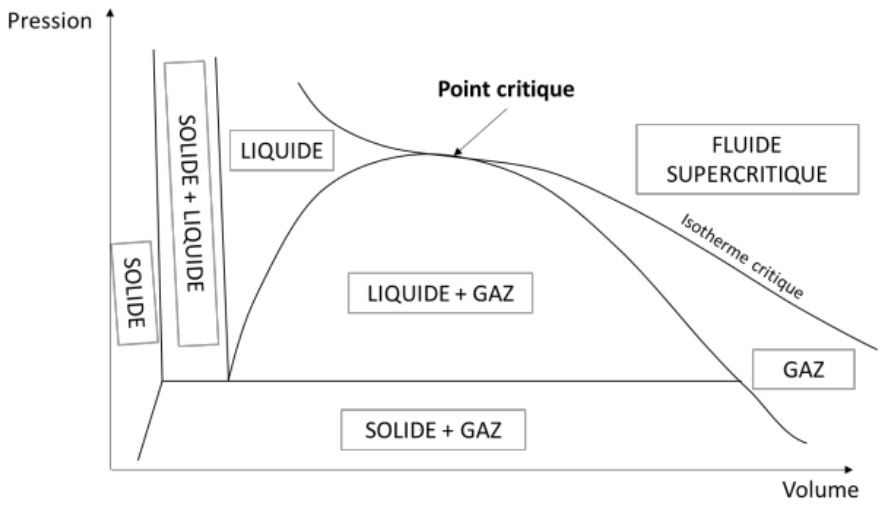
\includegraphics[width=\textwidth]{graphs/Clapeyron}
            }

                \vspace{-7pt}
                La pression de vapeur saturante $P_{vs}$ est la pression à laquelle le liquide et la vapeur sont en équilibre.\\
                $P_{vs}$ croit avec la température.


        \section{Mélange de corps pur}\label{sec:melange-de-corps-pur}

            \twoCol {
                Fraction molaire : $x_i = \dfrac{n_i}{x_{tot}}$
            }{
                Fraction massique : $w_i = \dfrac{m_i}{m_{tot}}$
            }
            \vspace{5pt}\\
            La masse molaire du mélange correspond à la moyenne pondérée des masses molaires des corps purs.\\
            On définis de même la pression partielle $P_i = x_i \times P$ où la loi des gaz parfaits s'applique aussi.


    \chapter{Le premier principe}\label{ch:le-premier-principe-de-la-thermodynamique}


        \section{Les différents types d’énergie}\label{sec:les-differents-types-denergie}

            \subsection{Chaleur et température}\label{subsec:chaleur-et-temperature}

                Un transfert de chaleur correspond à un échange d'énergie microscopique (transfert d'agitation thermique par chocs moléculaires), caractérisé par un changement de température ou d'état.

            \subsection{Énergie non calorifique : travail $W$}\label{subsec:energie-non-calorifique}

                \twoCol[61] {
                $\delta W = X_\re{ext}\ \re dx$, ou $W = \intt^{x_\re{final}}_{x_\re{initial}} X_\re{ext}\ \re dx$.\\
            }{
                \begin{itemize}
                    \item \underline{Travail mécanique :} $\delta W = F_{ext}\ \re d l$
                    \item \underline{Travail électrique :} \ $\delta W = E_{ext}\ \re d q$
                    \item \underline{Travail volumique :} $\delta W = - P_{ext}\ \re d V$
                \end{itemize}
            }

                \twoCol[61] {
                \vspace{-30pt}\\
                \resizebox{.49\textwidth}{!}{
                    \includestandalone[mode=buildnew,page=1, scale]{out/pv_diagram_1}
                }
                \resizebox{.5\textwidth}{!}{
                    \includestandalone[mode=buildnew,page=1, scale]{out/pv_diagram_2}
                }
            }{
                \vspace{5pt}
                Dans le cas d'une transformation réversible, comme le système est constamment à l'équilibre, la tension exercée par le milieu extérieur sera également la tension du système : $X_{ext} = X_\sigma$.
            }

                \vspace{-7pt}


        \section{Le premier principe}\label{sec:le-premier-principe}

            C'est le principe de la conversion de l'énergie : l’énergie ne peut être ni créée, ni détruite mais seulement transformée d’une forme en une autre.

            \twoCol {
                \vspace{-18pt}\\
                \begin{align*}
                    E_{totale} &= E_\re{c,macro} + E_\re{p,macro} + E_\re{c,micro} + E_\re{p,micro}\\
                    &= E_m + U
                \end{align*}
                \vspace{-18pt}
            }{
                Dans un système fermé :
                \vspace{4pt}\\
                $\Delta E_{totale} = \Delta U = Q + W$
            }
            \vspace{7pt}\\
            $E_\re{c,macro}$, $E_\re{p,macro}$ et $U$ sont des fonctions d'état (ne dépendent pas du chemin suivi), contrairement à $W$ et $Q$.\\

            \textbf{Application du premier principe à un système immobile à l'échelle macroscopique :}
            \vspace{4pt}\\
            Nous considérerons que la seule forme de travail échangé est due aux forces de pression : $W = \intt^{V_\re{f}}_{V_\re{i}} - P_\re{ext}\ \re dV$
            \vspace{4pt}
            \begin{itemize}
                \item \underline{Transformation isochores :} $W = 0$ et $Q$ ne dépend pas du chemin suivi car $\Delta U = Q$.
                \vspace{4pt}
                \item \underline{Transformation isobare :} Comme $P_{ext} = P_\sigma = \re{const}$, $\Delta U = Q - P_\re{ext} (V_f - V_i)$.\\
                On définis ainsi l'enthalpie $H = U + PV$.
                Lors d'une transformation isobare, $Q = \Delta H = \Delta U + P \times \Delta V$.
                \vspace{4pt}
                \item \underline{Transformation abiatique :} $Q = 0$ donc $\Delta U = W_{abia}$.
            \end{itemize}


        \section{Cas du gaz parfait}\label{sec:cas-du-gaz-parfait}

            \subsection{Coefficients calorimétriques des gaz parfaits}\label{subsec:coefficients-calorimetriques-des-gaz-parfaits}

                Toujours valide, car $W = 0$ pour une transformation isochore, et $U$ est une variable d'état :
                \[\Delta U = n \overline{C}_v \Delta T \quad\quad \Delta H = n \overline{C}_p \Delta T\]

                \underline{Relation de Mayer :} $C_p - C_v = nR$ ou $\overline{C}_p - \overline{C}_v= R$ et $\gamma = \dfrac{\overline{C}_p}{\overline{C}_v}$

            \subsection{Transformation adiabatique d'un gaz parfait}\label{subsec:transformation-adiabatique-d'un-gaz-parfait}
                Toute transformation adiabatique d’un gaz parfait s’accompagne d’un changement de température.\\
                \underline{Relations de Laplace :}
                \[P V^\gamma = const. \quad\quad T V^{\gamma - 1} = const. \quad\quad P T^\frac{\gamma}{\gamma - 1} = const. \]


    \chapter{Le second principe}


        \section{Limites du premier principe}

            Le premier principe permet de traduire le principe de la conservation de l'énergie, mais ne permet pas :
            \begin{itemize}
                \item d'expliquer pourquoi certains échanges d'énergie ou transformation sont spontanées alors que d'autres sont impossibles,
                \item de rendre compte de la qualité de l'énergie (le travail se transforme sans pertes en chaleur, alors que la chaleur se transforme en travail avec un rendement de $30\%$, on dit que la chaleur est une forme dégradée de l'énergie).
            \end{itemize}


        \section{Deuxième principe}

            \subsection{Définition de l'entropie}

                Tout comme nous avons $\delta W = X_\re{ext} \cdot \re d x$, on définie l'entropie $S$ par $\delta Q = T_\re{ext} \cdot \re d S$.\\
                Or, l'entropie est une fonction d'état (ne dépend que de l'état initial et final) :

                \[\re d S = \dfrac{\delta Q}{T_\re{ext}} = \dfrac{\delta Q_{rev}}{T_\re{ext}} \qquad \Delta S = \int_{E_\re{initial}}^{E_\re{final}} \dfrac{\delta Q_\re{rév}}{T_\sigma}\]

                L'entropie varie avec la quantité de chaleur transférée en supposant la transformation réversible.

            \subsection{Propriété de l’entropie}

                \twoCol {
                \underline{Pour une transformation réversible :}\\
                L'entropie du système $\sigma$ et de l'extérieur $\sigma_1$ sont opposées ($\delta Q$ opposés et températures identiques), donc l'entropie totale de l'univers $\sigma'$ (ou de $\{\sigma + \sigma_1\}$ isolé) est nulle : $\Delta S_{\sigma'} = 0$ car $\Delta S_\sigma = - \Delta S_{\sigma_1}$.
            }{
                \underline{Pour une transformation irréversible :}\\
                Les transferts $\delta Q$ sont toujours opposés, mais les températures ne sont pas les mêmes, ainsi, on a :\\
                $\Delta S_{\sigma'} = Q_\sigma \left( \dfrac{1}{T_\sigma} - \dfrac{1}{T_{\sigma_1} }\right)$.
            }

                Comme la chaleur va toujours du corps le plus chaud vers le plus froid (second principe), le second principe s'écrit aussi :
                l'entropie est créable et indestructible.

            \subsection{Enoncés du deuxième principe}

                \begin{itemize}
                    \item Pour une transformation irréversible (spontanée), l'entropie augmente.
                    \item Pour une transformation impossible (sans intervention extérieure), l'entropie diminue.
                    \item Pour une transformation réversible, l'entropie est nulle.\vspace{5pt}
                \end{itemize}
                On dit aussi qu'il est impossible de réaliser une transformation dont l'unique effet serait un transfert de chaleur d'un corps donné vers un corps plus chaud.

        \section{Signification physique et microscopique de l’entropie}

            On associe l'entropie au désordre moléculaire d'un système : on peut la définir à partir du nombre de micro-états (ou complexions) possible d'un système (positionnement particulier des atomes).\\
            L'entropie/le désordre augmente donc avec le volume, la température, et le mélange de plusieurs composants.\\

            L'entropie se définis $S = k_B \cdot \ln \Omega$ ($\Omega$ le nombre de micro-états et $k_B = \frac{R}{N_A}$ la constante de boltzmann).\\

            Pour un cristal parfait au zéro absolu, $\Omega = 1$, ainsi, le principe de Nernst ou troisième principe dit : l'entropie à $0K$ d'un corps à complexion unique est nulle.

        \section{Coefficient de performance et rendement}

            \[\re{CoP} = \dfrac{\re{Ce qui m'intéresse}}{\re{Ce que ça me coûte}} \hspace{60pt} r = \dfrac{\re{CoP}_\re{irrév}}{\re{CoP}_\re{rév}}\]

            Pour une machine thermique, $\re{CoP}$ et $r$ dépendent de $Q_1$ (source à température $T_1$), $Q_2$ (à $T_2$) et $W$.

\end{document}
